%%%%%%%%%%%%%%%%%%%%%%%%%%%%%%%%%%%%%%%%%%%%%%%%%%%
%% P3: Phenomenology of Particle Physics                         
%%
%% Author:  André Rubbia                   		 
%%
%% Figure 28.20 Predicted $y$-dependence of the differential cross-section of antineutrino scattering.
%%
%% This work is licensed under the Creative Commons Attribution 4.0 International License. 
%% To view a copy of this license, visit http://creativecommons.org/licenses/by/4.0/ or 
%% send a letter to Creative Commons, PO Box 1866, Mountain View, CA 94042, USA.
%%
%%%%%%%%%%%%%%%%%%%%%%%%%%%%%%%%%%%%%%%%%%%%%%%%%%%

\documentclass[a4paper,10pt]{article}

\usepackage[T1]{fontenc}
\usepackage[utf8]{inputenc}
\usepackage{lmodern}
\usepackage[labelfont=bf]{caption}
\usepackage{upgreek}

\usepackage{amssymb}
\usepackage{amsmath}
\usepackage{mathtools}

\usepackage{tikz}
\usepackage{pgfplots}
\pgfplotsset{compat=1.17}
\usepgfplotslibrary{ternary}
\usepgfplotslibrary{fillbetween}
\usepgfplotslibrary{external}

\def\d{\mathrm{d}}
\setlength{\oddsidemargin}{-1.0cm}
\setlength{\evensidemargin}{-1.0cm}
\setlength{\textheight}{25cm}
\setlength{\textwidth}{18cm}

\pgfkeys{/pgf/number format/.cd,1000 sep={}}

\begin{document}

%%%%%%%%%%%%%%%%   FIGURE  %%%%%%%%%%%%%%%%%%%%%%%%%%%%%%
\begin{figure}[htb]
	\centering
	\begin{tikzpicture}[scale=1]
\begin{axis}[
    title={Total neutrino cross-section},
    xlabel={Neutrino energy $E_\nu$ (GeV)},
    ylabel={$\sigma/E_\nu$ (cm$^2$/GeV)},
    height=8cm,
    xmin=0, xmax=250,
    ymin=0, ymax=1.,
   ymajorgrids=true,
    xmajorgrids=true,
   grid style=dashed,
   legend pos=outer north east
]

   %% CCFR NU
    \addplot[
    color=blue,
    mark=square*, only marks,
    error bars/.cd,
    y dir=both, y explicit
    ]
    coordinates {
(37.1,0.654)+-(0,0.022472205)
(44.7,0.621)+-(0,0.02236068)
(54,0.661)+-(0,0.019697716)
(63.5,0.664)+-(0,0.026)
(75.4	,0.664)+-(0,0.02912044)
(91,0.644)+-(0,0.058940648)
(111.7,0.659)+-(0,0.064845971)
(124.8,0.665)+-(0,0.042059482)
(141.2,0.695)+-(0,0.050249378)
(157.4,0.68)+-(0,0.037589892)
(165.1,0.714)+-(0,0.040311289)
(179.8,0.727)+-(0,0.039)
(190.8,0.749)+-(0,0.038078866)
(212.5,0.709)+-(0,0.05)
(229.1,0.756)+-(0,0.055027266)
    };

   %% CCFR ANU
    \addplot[
    color=blue,
    mark=square, only marks,
    error bars/.cd,
    y dir=both, y explicit
    ]
    coordinates {
(36.9,0.361)+-(0,0.018027756)
(45,0.352)+-(0,0.014764823)
(54,0.35)+-(0,0.014764823)
(63.8,0.332)+-(0,0.016643317)
(75.6,0.331)+-(0,0.021931712)
(89.3,0.333)+-(0,0.034438351)
(110.3,0.314)+-(0,0.040496913)
(126.5,0.341)+-(0,0.036235342)
(150,0.339)+-(0,0.026627054)
(174.4,0.321)+-(0,0.025806976)
(201.9,0.303)+-(0,0.031064449)
    };

   %% CDHS NU
    \addplot[
    color=magenta,
    mark=triangle*, only marks,
    error bars/.cd,
    y dir=both, y explicit
    ]
    coordinates {
(50,0.706)+-(0,0.002)
(82,0.700)+-(0,0.014)
(101,0.708)+-(0,0.008)
(121,0.710)+-(0,0.007)
(145,0.711)+-(0,0.007)
    };

   %% CDHS ANU
    \addplot[
    color=magenta,
    mark=triangle, only marks,
    error bars/.cd,
    y dir=both, y explicit
    ]
    coordinates {
(50,0.331)+-(0,0.005)
(82,0.335)+-(0,0.030)
(101,0.336)+-(0,0.016)
(121,0.337)+-(0,0.012)
(145,0.341)+-(0,0.012)
    };

\draw[thick,dashed] (axis cs: 0,0.677) -- +(axis cs: 250,0);
\draw[thick,dashed] (axis cs: 0,0.334) -- +(axis cs: 250,0);
\end{axis}
\end{tikzpicture}
	\begin{tikzpicture}[scale=1]
\begin{axis}[
    height=7cm, width = 5cm,
    symbolic x coords={xleft,CCFR,CHARM,FNAL-15',BEBC,CITFR,xright},
    xtick=data,
    xticklabel style={rotate=90},
    ymin=0, ymax=1.,
    ymajorgrids=true,
    xmajorgrids=true,
   grid style=dashed,
]


    \addplot[
    color=blue,
    mark=*, only marks,
    error bars/.cd,
    y dir=both, y explicit
    ]
    coordinates {
(CCFR,0.669)+-(0,0.024186773)
(CHARM,0.686)+-(0,0.0200998)
(FNAL-15',0.62)+-(0,0.05)
(BEBC,0.723)+-(0,0.038275318)
(CITFR,0.609)+-(0,0.039051248)
};
   \addplot[
    color=blue,
    mark=o, only marks,
    error bars/.cd,
    y dir=both, y explicit
    ]
    coordinates {
(CCFR,0.34)+-(0,0.020223748)
(CHARM,0.335)+-(0,0.0107703)
(FNAL-15',0.34)+-(0,0.029068884)
(BEBC,0.351)+-(0,0.018867962)
(CITFR,0.29)+-(0,0.019209373)
};
\draw[thick,dashed] (axis cs: xleft,0.677) -- (axis cs: xright,0.677);
\draw[thick,dashed] (axis cs: xleft,0.334) -- (axis cs: xright,0.334);
\end{axis}
\end{tikzpicture}
	\caption{Deep inelastic cross-section for neutrinos and antineutrinos.
	(left) Measurements on iron for neutrinos (closed symbols) and
	antineutrinos (open symbols) from CCFR~\cite{Blair:1983su} (squares) and CDHS~\cite{Berge:1987zw} (statistical error only -- triangles).
	(right) Slope measurements from other experiments.
	The slope data are from CCFR~\cite{Blair:1983su},
	CHARM~\cite{Allaby:1987bb},
	FNAL-15' bubble chamber~\cite{Baker:1982jf,Taylor:1983qj},
	BEBC~\cite{Bosetti:1981ip},
	CITFR~\cite{Barish:1977ny}.
	}
\end{figure}
%
%%%%%%%%%%%%%%%%   END FIGURE  %%%%%%%%%%%%%%%%%%%%%%%%%%%%%%
%
\begin{thebibliography}{99}
\bibitem{Blair:1983su}
R.~Blair {\em et~al.}, ``Measurement of the rate of increase of neutrino
  cross-sections with energy,'' {\em Phys. Rev. Lett.}, vol.~51, pp.~343--346,
  1983.

\bibitem{Berge:1987zw}
P.~Bergé {\em et~al.}, ``Total neutrino and anti-neutrino charged current
  cross-section measurements in {100-GeV, 160-GeV and 200-GeV Narrow Band
  Beams},'' Tech. Rep. CERN-EP/87-09, 1987.

\bibitem{Allaby:1987bb}
J.~Allaby {\em et~al.}, ``Total cross-sections of charged current neutrino and
  anti-neutrino interactions on isoscalar nuclei,'' {\em Z. Phys. C}, vol.~38,
  pp.~403--410, 1988.

\bibitem{Baker:1982jf}
N.~Baker {\em et~al.}, ``Measurement of the muon-neutrino charged current
  cross-section,'' {\em Phys. Rev. Lett.}, vol.~51, pp.~735--738, 1983.

\bibitem{Taylor:1983qj}
G.~Taylor {\em et~al.}, ``Anti-muon-neutrino nucleon charged current total
  cross-section for {5-GeV to 250-GeV},'' {\em Phys. Rev. Lett.}, vol.~51,
  pp.~739--742, 1983.

\bibitem{Bosetti:1981ip}
P.~Bosetti {\em et~al.}, ``Total cross-sections for $\nu_\mu$ and
  $\bar{\nu}_\mu$ charged current interactions between {20-GeV and 200-GeV},''
  {\em Phys. Lett. B}, vol.~110, pp.~167--172, 1982.

\bibitem{Barish:1977ny}
B.~Barish {\em et~al.}, ``Measurements of
  ${\ensuremath{\nu}}_{\ensuremath{\mu}}n$ and
  ${\overline{\ensuremath{\nu}}}_{\ensuremath{\mu}}n$ charged current total
  cross-sections,'' {\em Phys. Rev. Lett.}, vol.~39, p.~1595, 1977.
\end{thebibliography}


\end{document}
